
\chapter{基于传统特征与深度特征融合的无线调制方式识别技术研究}
\section{引言}
图像识别问题是计算机视觉领域要解决的基础问题,如果将图像看作一种模式,那么图像识别问题也是一种特殊的模式分类问题,包括早期的光学字符识别、生物特征识别中的人脸识别、指纹识别、虹膜识别,也包括场景识别、视频中的目标识别、动作识别等. 基于传统的模式分类方法,这类问题已经得到一定程度的解决,例如支持向量机、人工神经网络、近邻法等方法,通过特征提取、分类器训练过程得到分类器,输出分类结果. 但是,传统的模式分类方法通常基于人工设计的特征,经过特征提取算法得到原始图像的特征数据,例如颜色特征、SIFT 特征、HOG 特征、HOF 特征、GIST 特征等,而这些特征数据却存在类内方差较小而类间方差较大的问题.因为一种特征通常只对图像部分特性的变化较为敏感,而对其他特性的变化不敏感,所以,当两类图像的差异在某种特征敏感特性上的差异不大时,基于单一特征训练的分类器就无法输出正确的分类. 除此之外,图像中复杂的背景噪声也会导致特征数据质量下降,既增加分类器训练的难度,又降低分类的准确性.

得到原始图像的特征数据,例如颜色特征、SIFT 特征、HOG 特征、HOF 特征、GIST 特征等,而这些特征数据却存在类内方差较小而类间方差较大的问题.因为一种特征通常只对图像部分特性的变化较为敏感,而对其他特性的变化不敏感,所以,当两类图像的差异在某种特征敏感特性上的差异不大时,基于单一特征训练的分类器就无法输出正确的分类. 除此之外,图像中复杂的背景噪声也会导致特征数据质量下降,既增加分类器训练的难度,又降低分类的准确性.解决这种问题的一种思路就是使用特征融合方法,同时提取多种特征进行分类器训练,实现特征互补,降低单一特征固有缺陷的影响. 特征融合方法的思想来源于早期的信息融合( information fusion)领域,它的数据主要来源于多种传感器,用于军事领域的多传感器融合. 早期信息融合的基础理论主要包括模糊集、证据理论等,后来信息融合在民用领域得到了较快的发展,尤其是在生物安全认证方面[1],进行多生物特征的融合识别. 目前在学术界被公认的信息融合层次划分为分类器级( 决策级) 、特征级和数据级,处理数据的维度和总量依次升高.在模式识别领域,受到计算机运算能力的限制,早期的研究主要集中在分类器级的融合算法,例如,Kittler
等[2]提出的基于贝叶斯决策理论的分类器融合框架,为以后的研究奠定了良好的基础. 近年来,随着人工智能技术的发展,特征融合成为研究热点,特别是在图像识别问题中得到了广泛的应用.

\section{传统特征}
\subsection{基本时频特征}
时间特征\par

频率特征\par

\subsection{高阶累积量}
四阶累积量\par

六阶累积量\par

\subsection{专家循环矩特征}
基于综合循环矩特征[1]目前广泛流行的调制识别和形成分析导出的决策树调制分类到不同的类别。 一般来说,它们采用方程 \ref{subsec:eq1} 给出的形式。
\begin{equation}
	\label{subsec:eq1}
	snm = f_{m}(x^{n}(t)...x^{n}(t + \tau))
\end{equation}
通过计算关于瞬时或时间延迟的接收信号$r(t)$的$n$次方的第$m$阶统计量,我们可以获得一组统计量,该统计量在给定特征的决策过程的情况下将其与其他调制方式唯一地分开。 对于我们的专家功能集,我们计算32个功能。 这些由0和8个样本的循环时间滞后组成。 复数接收信号的前2个功率的前2个时刻,每个时滞的幅度,相位和相位的绝对值。\par

\section{特征融合理论}
特征融合在信息融合中属于中间层次的融合,信息融合理论是特征融合的基础理论.信息融合是对多源异构数据进行综合处理,从而达到联合决策的目的.其实,人类对事物的认知过程就是对多源信息的融合过程[3],人们每时每刻都在通过视觉、听觉、触觉、嗅觉、味觉等多种感官接收各种各样的信息,这些信息转化成了神经脉冲信号传输到大脑皮层进行综合决策.实际应用中,由于多源数据的结构和含义不同,在处理时不能一概而论,必须经过融合算法处理.在计算机视频和模式识别领域,使用特征融合方法解决图像识别问题,就是基于信息融合思想,通过融合算法使用图像多角度、多层次的特征(图像的颜色、形状、梯度)、空间特征和时间特征、全局特征和局部特征等,来实现更智能的图像信息处理.

随着学术研究的推进,信息融合的数据来源更加多样,应用的领域也更加广泛,特别是CPU、GPU计算性能的显著提升,大规模分布式计算、并行计算模型进一步发展,人类能够对大数据进行快速处理,这使得信息融合的研究从分类器级推进到了特征级和数据级的层面.如果将图像识别问题看作模式分类问题,那么使用特征融合方法主要基于2个基本的经验性假设:1) 融合多特征通常比单一特征具有更好的分类性能;2) 进行融合的多种特征之间相关性较小.前者是应用该方法的出发点和基础思想,后者对于图像多特征的选择具有指导意义.应当从多个角度选择相关性尽量小的特征参与特征融合,才能发挥该方法的优点,实现特征互补.特征融合方法直接作用在特征上面,它的优点在于可以直接利用已有的特征提取算法提取特征,相对于重新设计特征和特征提取算法,其花费的代价更低.

模式分类问题的解决过程一般包括数据获取、预处理、特征提取、分类器设计与训练和分类决策等步骤,如图 1所示,信息融合的3个层次恰好可以与这个过程对应.特征保留了必要的、显著的信息,既降低原始数据的冗余性,减少数据噪声,又比分类器决策结果有更充分的数据信息,数据量和数据维度适中,因此在这个层次上进行融合是目前最优的选择.引入特征融合方法的模式分类问题可以表述为,定义模式空间Ω={ω1, ω2, …, ωc}和样本集合X,其中ωk表示一个模式类,X中每个元素Xj是一个样本的特征集合,其中j∈[1, P],P为样本总数;特征集合Xj={Xj1, Xj2, …, XjD}表示样本有D种特征,样本特征向量Xji={xj1i, xj2i, …, xijni}∈Xj,xjnii表示样本第种i特征的一个维度,ni是这种特征的维度,N=∑1D∑1Dni,为样本特征总体维度;基于特征融合的模式分类问题就是得到样本特征集合Xj到ωk的对应关系,记为f:Xj→ωk.

\section{基于深度学习的特征融合算法}
深度学习理论是在人工神经网络的基础上发展起来的机器学习理论,在多层神经网络中加入了更多隐层单元,得到了深度神经网络模型. 其中深度卷积神经网络模型是该理论中的重要模型之一. 使用该模型可以进行有监督地学习,将特征提取过程
与分类器训练过程整合在一起,实现端到端的机器学习. 基于深度学习理论的特征融合算法是将特征融合的思想引入深度神经网络模型,使用多特征输入到模型中进行训练,在模型中选择 2 个隐层进行特征融合.

Simonyan 等[16]首先提出了一种使用双流架构的深度卷积神经网络模型,可解决视频中的动作识别问题. 该模型分别建立一个空间流卷积神经网络和一个时间流卷积神经网络进行独立训练,在最终的 Softmax 分类输出层将这 2 个网络进行融合,属于分类器级的融合. 而 Feichtenhofer 等[15]则在这个基础上改进了网络融合方法,提出了空间特征融合方法和时间特征融合算法,不仅可以在 Softmax 层进行融合,还可以在卷积层之后的 ReLU 层进行融合,实现特征级的融合.
\subsection{空间特征融合算法}
空间特征融合算法可以对卷积层输出的 2 个特征图( feature map) 进行融合,得到融合后的特征图,从而将 2 个深卷积神经网络模型连接在一起,这个连接点就是融合点. 因此,引入特征融合方法之后,2 个深卷积神经网络模型在融合点之前分别进行特征学习,并在融合点将独立学习的特征进行融合,最后开始共同学习. 融合函数定义为
f∶ xa
t + xb
t →yt ( 19)
其中: xat 和 xb
t 表示 t 时刻的视频帧分别经过卷积运算得到的空间特征图,yt 表示融合空间特征图,xa、xb、yt∈RHWD而 H、W 和 D 分别表示特征图的长度、宽度和通道数量. 融合函数包含加性融合函数、最大融合函数、级联融合函数、卷积融合函数和双线性
融合函数等.加性融合函数 ysum = fsum ( xa,xb) ,是对 2 个特征图对应位置元素的值进行相加,如式( 20) 所示,融
合特征图的通道数不变,其中 i∈[1,H],j∈[1,W],d∈[1,D].ysumi,j,d = xa
i,j,d + xbi,j,d ( 20)最大融合函数 ymax = fmax ( xa,xb) 与加性融合函数相似,是将 2 个特征图对应的位置元素值较大的一个作为融合结果,即ymaxi,j,d = max{ xa	i,j,d,xb	i,j,d } ( 21)级联融合函数 ycat = fcat ( xa,xb) 与前两者不同,它保留了 2 个特征图的结果,并将融合后特征图的通道数变为原始特征图的两倍,如ycati,j,2d = xai,j,d,ycat
i,j,2d - 1 = xbi,j,d ( 22)其中 y∈RH × W × 2D.卷积融合函数 yconv = fconv ( xa,xb) ,是将级联融合函数的融合结果与滤波器 f 进行卷积运算,并且引入偏差值 b,从而实现融合特征图的降维处理. 表示为yconv = ycatf + b ( 23)其中 f∈R1 × 1 × 2D × D,b∈RD.

双线性融合函数 ybil = fbil ( xa,xb) ,是对 2 个特征图对应的位置元素进行外积运算后求和,融合特征图的通道数是原始特征图通道数的平方,表示为ybil = ∑Hi = 1∑Wj = 1xaTi,jxbi,j ( 24)其中 ybil∈RD2. 这种融合函数常被用在 ReLU 层,能够对 2 个特征图对应通道进行融合.

\subsection{时间特征融合算法}

时间特征融合算法主要作用在深度卷积神经网络的池化层. 在进行池化处理之前,需要将空间特征图按照时序进行堆叠,使得输入池化层的特征图维度提高,表示为 x1,…,T∈RHWTD. 文献[15]提出了3D 池化方法和 3D 卷积 + 3D 池化方法,直接保留了时序信息.3D 池化方法是对深度卷积神经网络中通常使用的 2D 池化方法的直接扩展,使用 HWT 的 3D 池化立方代替原始池化层的计算方法,对输入的特征图 x进行池化运算,从而将池化处理从空域扩展到时域. 3D 池化立方可以使用最大池化方法,保留立方区域中的最大值作为池化结果. 这种方法是对特征图的单通道进行处理,不进行跨通道的池化运算.3D 卷积 + 3D 池化方法则是在 3D 池化方法基础上,再加入一个滤波器 f∈RH'W'T'DD'和偏差值 b,对输入的特征图 x1,…,T进行卷积运算,如y1,…,T = x1,…,T * f + b ( 25)计算得到的 y1,…,T再进行 3D 池化处理. 使用滤波器 f 可以在一个局部的时空邻域内对图像特征的组合,通过使用H'W'T'D的卷积核进行卷积运算,增加模型的连接权重数量.在处理视频数据时,时间特征融合算法通常与空间特征融合算法同时使用,通过利用视频中的时序信息,提高基于视频的动作识别或者目标识别的准确率.
\section{传统特征与深度特征融合框架}

\subsection{基于LR的融合框架}
\begin{figure}[!h]
	\centering
	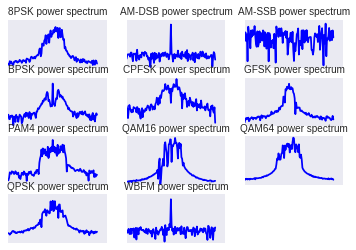
\includegraphics[scale=0.9]{figures/chapter_3/signal_view_2}
	\caption{sigmoid函数与tanh函数}\label{fig_2_2}
\end{figure}

\subsection{基于DNN的融合框架}
\begin{figure}[!h]
	\centering
	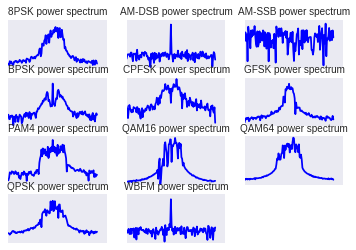
\includegraphics[scale=0.9]{figures/chapter_3/signal_view_2}
	\caption{sigmoid函数与tanh函数}\label{fig_2_2}
\end{figure}

\subsection{基于集成树的融合框架}
\begin{figure}[!h]
	\centering
	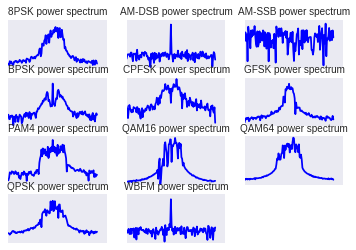
\includegraphics[scale=0.9]{figures/chapter_3/signal_view_2}
	\caption{sigmoid函数与tanh函数}\label{fig_2_2}
\end{figure}


\section{结果及分析}

\begin{figure}[!h]
	\centering
	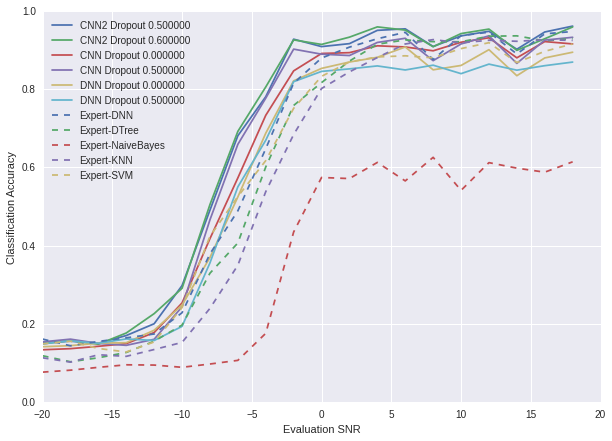
\includegraphics[scale=0.3]{figures/chapter_3/result}
	\caption{sigmoid函数与tanh函数}\label{fig_2_2}
\end{figure}

\subsection{学习概论}
为了验证这一理论,学习歧视性特征可能推广和帮助歧视新的未知调制在半监督的方式使用bootstrap方法,
我们重复我们的先前的方法,但这次我们训练监督分类器11调制9。
我们支持BPSK和16QAM调制,在监督培训期间不提供关于这些类别或其示例的信息。
然后,我们从所有11个类中举例,将它们转换成压缩的特征映射空间,并使用图8中所示的t-SNE可视化二维嵌入。\par

仔细检查这些结果,我们可以看到BPSK不幸与QPSK和8PSK调制(它是其中的一个子集)相当混杂。
然而,QAM16是一个以前看不见的类,这些特征在QAM64附近紧密聚集在一个相当明确的可分离的嵌入空间区域。
这些结果虽然非常初步和定性,但确实支持这一事实,即自举特征映射具有显着的泛化能力,
能够识别,聚类和辨别新的未知的或以前看不见的调制类型,但是并不保证在所有情况下都具有清晰的可分离性。
我们希望随着类别和特征数量的增加,这种泛化将会得到改善。
推进这一研究领域的挑战之一将是确定和量化特征总结能力的衡量标准,并着力于改进这一指标。\par

\subsection{未来应用-聚类}
一旦示例在嵌入空间中形成相对可分的簇,我们可以使用任意数量的聚类算法来将它们中的每一个分组并将其分配给类标签。在图9中,我们展示了一个使用DBSCAN [4]聚类算法的例子,将聚类分成一组未知但不同的调制类。我们发现这种聚类方法比较适合在我们的压缩空间中形成的不明确形状的聚类。聚类之后的数据处理可以包括标记许多示例的集群而不是每个单独的示例,从而提供从数据保存时间的效率提高的数量级。在包含许多类和例子的非常大的数据集上,这使得管理大规模学习任务比其他方法更容易处理。\par
虽然这些集群并非没有错误,但是在这个例子中,通常我们可以找到从发现的类集合到不同的真实命名类的一对一或多对一的映射。这保证了这样一种方法可以在将来用于快速组织和标记大量的无线电发射,并利用关于发射器类别特征的先前知识,但是仍然允许随着时间的推移识别系统能力,特征和类别标签的缩放最大限度地减少这样做所需的人力劳动。\par


\section{本章小结}
在这项工作中,我们已经证明,使用原始采样无线电时间序列数据上的卷积神经网络学习的低级别时间序列特征可以用于有效地聚类许多无线电信号调制类型,而没有明确标记的训练数据。我们已经表明,通过利用从差异特征映射和压缩重构空间学习的压缩表示,我们可以开始组织和构造复杂的无线电信号数据集与未标记或标记不佳的起点。这是一个强有力的结果,因为它展示了一个潜在的前进方向,可以学习区分,推理,回忆和描述新的和未知的无线电信号,而无需手动指导或专家指导。这是一个关键的要求,因为我们试图建立随着时间的推移而从经验中扩展能力的系统。将压缩的特征空间基础推广到新的信号类型仍然是这个领域的一个关键挑战,但是我们在这项工作中已经表明,在某些情况下这种特征泛化确实发生。展望未来,量化和优化这种效应的尝试将是重要的。\par

特征融合方法是模式识别领域的一种重要方法. 计算机视觉领域的图像识别问题作为一种特殊的模式分类
问题,仍然存在很多挑战. 特征融合方法能够综合利用多种图像特征,实现多特征的优势互补,获得更加鲁棒和准
确的识别结果. 笔者基于信息融合理论分析了特征融合方法的原理,介绍了特征融合方法的研究现状,讨论了特征
融合与 3 类主流基础理论相结合的方法,其中基于贝叶斯理论的特征融合算法可以实现多特征的融合决策,基于
稀疏表示理论的特征融合算法能够得到多特征的联合稀疏表示,基于深度学习理论的特征融合算法能够强化深度
神经网络模型的特征学习过程.\par
